% !TeX root = ../main.tex
% Add the above to each chapter to make compiling the PDF easier in some editors.
\chapter{Concept}\label{chapter:Concept}
The main draft of the project will be to run an app on a device, providing a camera. Running the life feed of the camera, speed signs should be detected and classified correctly, then this received information is passed to a driving simulator, steering an autonomous car. As soon as the simulator receives the required speed limit, the velocity is being adjusted. 
\begin{figure}[H]
	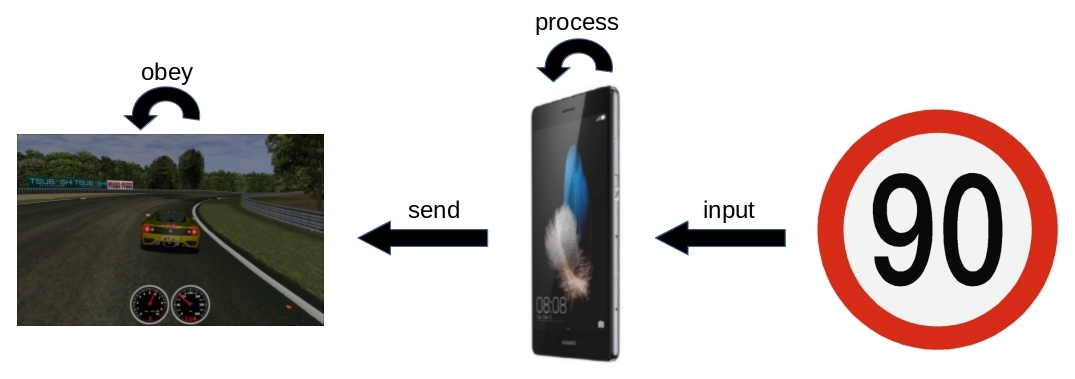
\includegraphics[width=\linewidth]{images/concept.jpg}
	\caption{Concept visualized}
\end{figure}

Komponentendiagramm\newline

The task of looking at a picture and telling what is in it, is quite trivial to humans and would usually not pose a challenging task to perform, whereas it is not that simple to computers. In order to classify images, or more exactly the objects comprised, machines ordinarily need a certain amount of preprocessing to extract characteristic Features. It is possible to summarize the smaller steps of the process into the two bigger, more generalized, steps of feature extraction and classification.



\section{Detection}
\begin{figure}[H]
	\minipage{0.33\textwidth}
	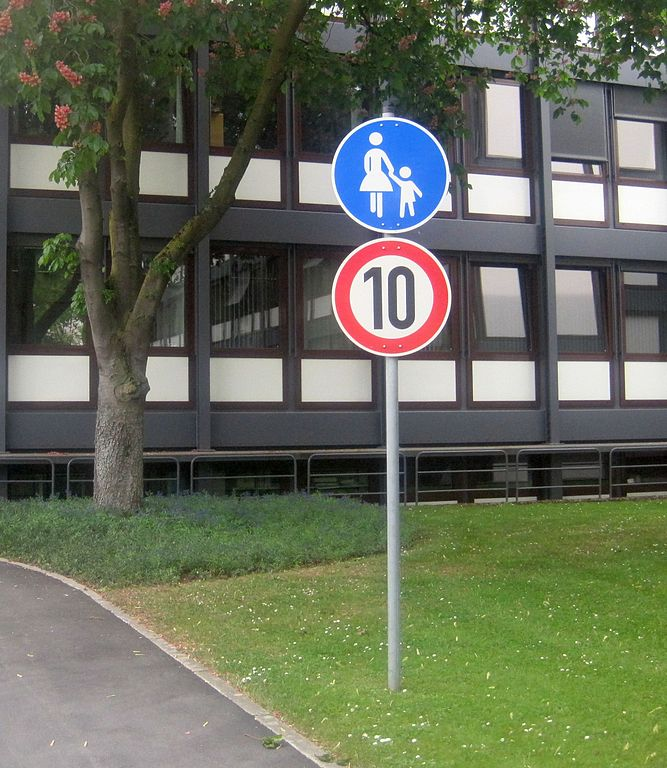
\includegraphics[width=\linewidth]{images/101.jpg}
	\caption{Original image \protect\footnotemark}\label{fig:original_image10}
	\endminipage\hfill
	\minipage{0.33\textwidth}
	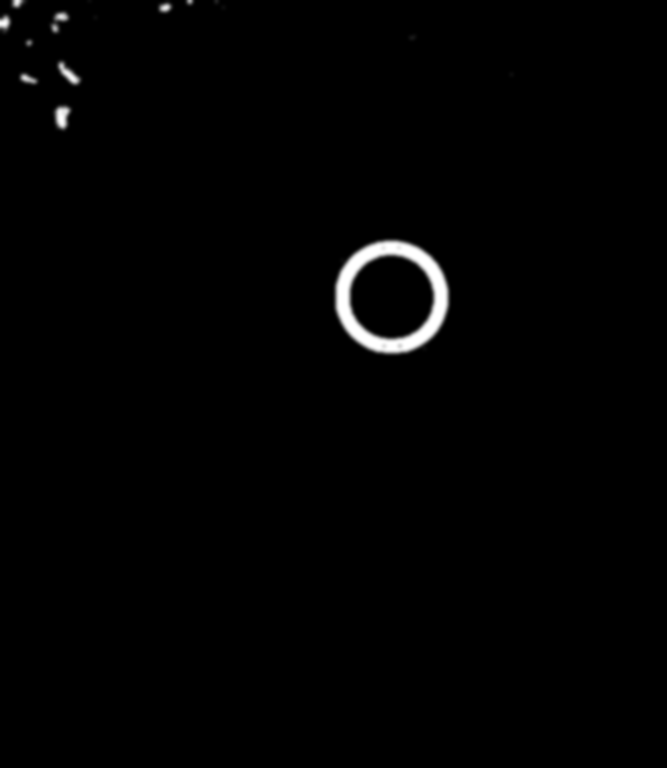
\includegraphics[width=\linewidth]{images/filteredimg.png}
	\caption{Filtered Image}\label{fig:red_filtered_image}
	\endminipage\hfill
	\minipage{0.33\textwidth}%
	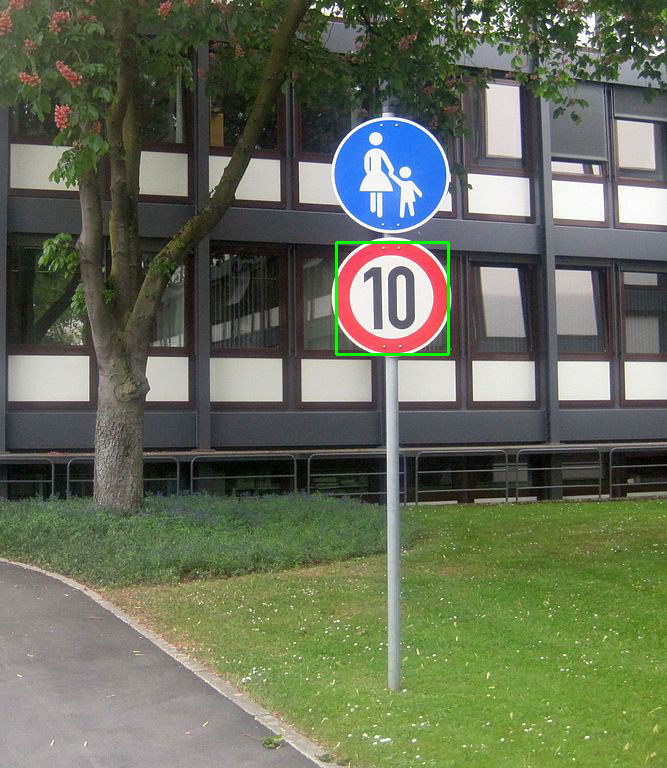
\includegraphics[width=\linewidth]{images/detectedimg.png}
	\caption{Detected image}\label{fig:detected_image}
	\endminipage
\end{figure}

\footnotetext{\url{https://goo.gl/Q6doij} (visited on 02.14.2018)}

Before we pass data through to the Classification phase, it is a reasonable step in the Program, to specify a Region Of Interest, with regard to saving some processing power. In order to specify ROIs, advantage was taken of the red circle around European Speed signs, the main steps of this part are to filter every red pixel out of the original image (Figure: \ref{fig:red_filtered_image}), subsequently an algorithm checks the filtered image for circles (Figure: \ref{fig:detected_image}). Filtering red pixels from a picture is no big sorcery, so this part is going to be skipped for now to come back later to this in the implementation section. The real gist of this step is to search an image for circles, therefore a common method used is the Circle Hough Transform. 

\subsection{Circle Hough Transform}
The Circle Hough Transform is a special case of the Hough transform, which determines lines in an image through Edge Detection Algorithms \cite{circlehough}. There are two slightly different Circle Hough Transforms, the first is only able to find circles of fixed radial size, the second is generally capable of finding Circles of any size. At first the variant with the fixed radius  of the algorithm is being explained, successively this method is being extended to the second, more generalized form of said algorithm.

\subsubsection{Fixed Radius}
First of all the image is being Converted to a binary image  (Figure: \ref{fig:binary_image}), further it is being processed via edge detection to determine every visible edge contained in the photo (Figure: \ref{fig:edge_detected_image}).
After this, the actual core of the Algorithm is being executed. Therefore an Accumulator Matrix is initialized with zeros. As the radius of the circle is considered constant, every ring in the picture can solely be described by two variables, their x and y coordinates, therefore the helping Accumulator Matrix is 2-Dimensional.
Above-mentioned Matrix can be pictured as a grid over the original image, where single pixels can be combined to bigger baskets. Now every basket or pixel of a detected edge (Figure: \ref{fig:edge_detected_image}) becomes the center of a new circle, with given fixed radius. After this each pixel that got "cut" by the circle gets incremented or up-voted in corresponding Accumulator Matrix. (Figure \ref{fig:circlehough_explanation}) Visualizes the voting steps, by displaying the green, red and blue circle as single examples of voting. The baskets or pixels with the highest votes can be considered to be centers of circles \ref{fig:voted_image}).
\newline

\begin{figure}[H]
	\minipage{0.47\textwidth}
	
\includegraphics[width=\linewidth]{images/circles.jpg}
	\caption{Binary image\protect\footnotemark
	}\label{fig:binary_image}
	\endminipage\hfill
	\minipage{0.47\textwidth}
	
\includegraphics[width=\linewidth]{images/circle_edges.jpg}
	\caption{Edge detected\protect\footnotemark}\label{fig:edge_detected_image}
	\endminipage\newline
	\minipage{0.47\textwidth}%
	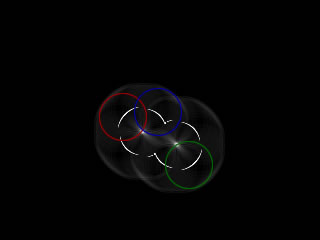
\includegraphics[width=\linewidth]{images/circlehough_explanation.jpg}
	\caption{Voting process visualized\protect\footnotemark}\label{fig:circlehough_explanation}
	\endminipage
	\hfill
	\minipage{0.47\textwidth}%
	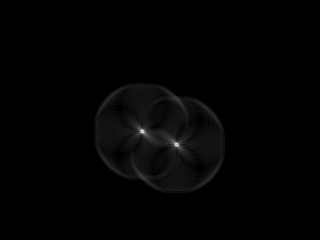
\includegraphics[width=\linewidth]{images/hough_circle.jpg}
	\caption{Voted image\protect\footnotemark}\label{fig:voted_image}
	\endminipage
	
\end{figure}
\setcounter{footnote}{2}
\footnotetext{\url{http://www.aishack.in/static/img/tut/circles.gif} (visited on 02.14.2018)}
\setcounter{footnote}{3}
\footnotetext{\url{http://www.aishack.in/static/img/tut/circle\_edges.jpg} (visited on 02.14.2018)}
\setcounter{footnote}{4}
\footnotetext{\url{http://www.aishack.in/static/img/tut/circlehough\_explanation.jpg} (visited on 02.14.2018)}
\setcounter{footnote}{5}
\footnotetext{\url{http://www.aishack.in/static/img/tut/hough\_circle.jpg} (visited on 02.14.2018)}

\subsubsection{Variable Radius}
A circle on a two-dimensional plane can be described by following formula[10]: \[ (x - a)^2 + (y - b)^2 = r^2  \]
, meaning the circle can be represented by the parameters (a, b, r), where "a" and "b" are the 2-Dimensional coordinate values representing the center of the circle, whereas the variable "r" provides the radius of given ring. \newline
The preprocessing (Figure: \ref{fig:binary_image} and Figure: \ref{fig:edge_detected_image}) is identical to the fixed-radius Circle Hough Transform, but what makes the difference now is, our Accumulation Matrix gains another Dimension, from having variable radii, therefore it is 3-Dimensional now. Usually a range for the radiuses is being defined to make things a little easier. Now the voting happens exactly as it would with the algorithm described before, but this time with the difference, that it has to be done with every radius in the before determined range. The center of the potential circles are now the ones with the most voted radii in all radius-dimensions.

\section{Classification}
In the project a decision was made, the scope of signs should be from 10 to 90 km/h, to reduce the amount of input data, needed to be provide, this range could be extended easily, by adding output Neurons and broaden the data set classes, used to train the Artificial Neural Network. \newline\newline
Preceding stage delivers an image of fixed size, that needs to be categorized into one out of 10 groups, these are the Speed limits "10km/h", "20km/h",..., "90km/h" and "no sign". To gain these information about the sub-image of the original image, the decision mas made to apply a Feed Forward Deep Neural Network. Said Neural Network is fed each individual pixel, provided by the ROI to its input neurons, the trained Model then outputs a prediction on what class the input picture might belong to.
\newline

\subsection{Model}
When coming up with determining an own model for classification purposes, it was relatively trivial to define the number of output neurons, as They just had to be the number of different signs, plus an additional neuron for signalizing, given input image can not be classified as a sign, this leaves the network with 10 neurons in our output layer. Generally the more neurons a model has, the more calculation operations have to be performed, when calculating a prediction.\newline
As the categories of signs, the net should specialize on, were all circular, it made sense, to accept a square image as input. Therefore the number of neurons, included by the input layer had to be a square number, as they represent the pixels fed by the image. Comparable datasets/classifiers, like NIST or MNIST\footnote{\url{http://yann.lecun.com/exdb/mnist/} (visited on 02.14.2018)} use 20x20 respectively 28x28 pixels. These datasets are established ones, that are used to train classifiers for recognizing handwritten digits. With regard to the more or less limited processing power of Android phones, the 20x20 format was taken over, demanding 400 neurons for the input layer. \newline
A NN is referred to be "deep", as soon as it contains more than one hidden layer on the inside.
Since the aim was to create a deep Neural Network with the limitations of running it in real time on an Android device, two input layers have been chosen. The amount of neurons in each layer was once again chosen with regard to the performance claims and set to 100 each.\newline
What needs to be said about the simplified visualization of my model(Figure:\ref{fig:neuralnetmodel}) is, not every connection between the neurons is presented in the figure. Obviously every arrow to the next layer is symbolic for a connection from said neuron to every neuron from the subsequent layer, and of course it was not possible to represent every node in each layer.

\begin{figure}[H]
	\centering
	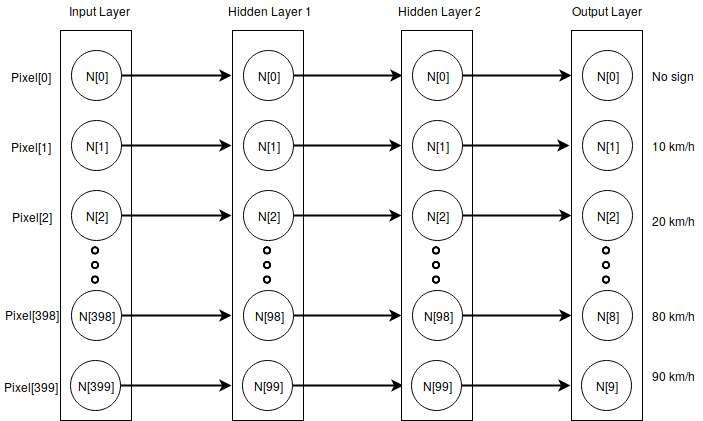
\includegraphics[width=0.9\linewidth]{images/neuralnetmodel.jpg}
	\caption{Simplified representation of the Neural Network Model }\label{fig:neuralnetmodel}	
\end{figure}
